\chapter{Simulaciones}
%-----------------------------------
%   SIMULACIONES
%-----------------------------------
\label{ch:simulaciones}

Debido a que no es factible implementar una red vehicular para poner a prueba el
protocolo de enrutamiento propuesto, la evaluación se hizo mediante
simulaciones. Se recurrió a la herramienta SUMO para modelar y simular el flujo
de vehículos por las calles \cite{SUMO}. Para simular la comunicación entre
vehículos y \textit{hosts}, se usó OMNET++, un simulador de eventos discretos
con el que se pueden evaluar protocolos de comunicaciones \cite{OMNeT}. Este se
utilizó en conjunto con el \textit{framework} INET, que proporciona modelos de
simulación de muchos protocolos estándar, como los protocolos de la pila TCP/IP
\cite{INET}. Para simular la red vehicular, se utilizó el \textit{framework}
Veins, que permite la interacción entre la simulación de los vehículos de SUMO y
la simulación de comunicaciones de OMNeT++ \cite{Veins}. Otras herramientas que
se utilizaron fueron el programa JOSM, para descargar y acondicionar mapas de
OpenStreetMap para realizar de las simulaciones de SUMO \cite{OpenStreetMap}
\cite{JOSM}, y QGIS, para la creación de la base de datos de redes viales.

En este capítulo, se explica cómo se utilizaron estas herramientas para el
desarrollo de las simulaciones que se llevaron a cabo para evaluar el desempeño
del protocolo propuesto. El código fuente, scripts y otros recursos se  pueden
consultar en el siguiente repositorio:

\begin{center}
\href{https://gitlab.com/Comecacahuates/simulacion-protocolo-erutamiento}
{https://gitlab.com/Comecacahuates/simulacion-protocolo-erutamiento}
\end{center}

\section{Instalación de las herramientas}
%-----------------------------------
%	INSTALACIÓN DE LAS HERRAMIENTAS
%-----------------------------------
\label{sec:instalacion_herramientas}

En esta sección, se explica cómo instalar las herramientas utilizadas para
realizar las simulaciones en el sistema operativo Debian Buster, que se utilizó
para el desarrollo del proyecto.

\subsection{Instalación de SUMO}
%-----------------------------------
%   INSTALACIÓN DE SUMO
%-----------------------------------
\label{subsec:instalacion_sumo}

Primero, se descarga el
\href{https://sourceforge.net/projects/sumo/files/sumo/}{código fuente de SUMO
1.8.0}, y se descomprime el directorio {\lstinline[language=bash]!sumo-1.8.0!}
dentro del directorio {\lstinline[language=bash]!~/src!}. Después, se instalan
los paquetes requeridos con el siguiente comando:

\begin{lstlisting}[language=bash]
$ sudo apt-get install ccmake python g++ libxerces-c-dev libfox-1.6-dev \
    libgdal-dev libproj-dev libgl2ps-dev
\end{lstlisting}

El código fuente se compila ejecutando los siguientes comandos:

\begin{lstlisting}[language=bash]
$ cd ~/src/sumo-1.8.0
$ export SUMO_HOME=$HOME/src/sumo-1.8.0
$ mkdir build/cmake-build
$ cd build/cmake-build
$ cmake ../..
$ make -j $(nproc)
\end{lstlisting}

Para que SUMO y las herramientas que incluye estén disponible en la variable de
entorno {\lstinline[language=bash]!PATH!} permanentemente, se agregan las
siguientes líneas al archivo {\lstinline[language=bash]!~/.bashrc!}:

\begin{lstlisting}[language=bash]
export SUMO_HOME=$HOME/src/sumo-1.8.0
export PATH=$SUMO_HOME/bin:$PATH
export PATH=$SUMO_HOME/tools:$PATH
\end{lstlisting}

Las instrucciones de compilación detalladas se pueden consultar en
\cite{CompilacionSUMO}.

% TODO: Escribir la evaluación de protocolos de enrutamiento: \cite{Nishat2011}.

\subsection{Instalación de OMNeT++}
%-----------------------------------
%	INSTALACIÓN DE OMNET++
%-----------------------------------
\label{subsec:instalacion_omnet}

Primero, se descarga el \href{https://omnetpp.org/download/}{código fuente de
OMNeT++ 6.0}, y se descomprime el directorio
{\lstinline[language=bash]!omnetpp-6.0pre10!} dentro del disrectorio
{\lstinline[language=bash]!~/src!}. Después, se instalan los paquetes
requeridos con el siguiente comando:

\begin{lstlisting}[language=bash]
$ sudo apt-get install build-essential clang lld gdb bison flex perl \
    python3 python3-pip qt5-default libqt5opengl5-dev libxml2-dev \
    zlib1g-dev doxygen graphviz libwebkit2gtk-4.0-37 \
    openmpi-bin libopenmpi-dev
$ python3 -m pip install --user --upgrade numpy pandas matplotlib \
    scipy seaborn posix_ipc
\end{lstlisting}

El código fuente se compila ejecutando los siguientes comandos:

\begin{lstlisting}[language=bash]
$ cd ~/src/omnetpp-6.0pre10
$ source setenv
$ ./configure WITH_OSG=no WITH_OSGEARTH=no
$ make
\end{lstlisting}

Para que OMNeT++ esté disponible en la variable de entorno
{\lstinline[language=bash]!PATH!} permanentemente, se agrega la siguiente línea
al archivo {\lstinline[language=bash]!~/.bashrc!}:

\begin{lstlisting}[language=bash]
export PATH=$HOME/src/omnetpp-6.0pre10:$PATH
\end{lstlisting}

Las instrucciones de compilación detalladas se pueden consultar en
\cite{CompilacionOMNeT}.

\subsection{Instalación de QGIS}
%-----------------------------------
%   INSTALACIÓN DE QGIS
%-----------------------------------
\label{subsec:instalacion_qgis}

Para instalar QGIS 3.10, se ejecutan los siguientes comandos:

\begin{lstlisting}[language=bash]
$ sudo apt-get install qgis qgis-plugin-grass
\end{lstlisting}

Se pueden consultar más detalles sobre la instalación en
\cite{InstalacionQGIS}.

\subsection{Instalación de JOSM}
%-----------------------------------
%	INSTALACIÓN DE JOSM
%-----------------------------------
\label{subsec:instalacion_josm}

JOSM es una aplicación Java, por lo que primero se debe instalar la máquina
virtual de Java con el siguiente comando:

\begin{lstlisting}[language=bash]
$ sudo apt-get install openjdk-11-jdk
\end{lstlisting}

Después, se descarga el archivo
\href{https://josm.openstreetmap.de/wiki/Download}{\code{josm-tested.jar}}, y
la aplicación se ejecuta con el siguiente comando:

\begin{lstlisting}[language=bash]
$ java -jar josm-tested.jar
\end{lstlisting}

Se pueden consultar más detalles en \cite{DescargaJOSM}.

\section{Base de datos de redes viales}
%-----------------------------------
%   BASE DE DATOS DE REDES VIALES
%-----------------------------------
\label{sec:creacion_base_de_la_datos_de_redes_viales}

Para cada red vial, se utilizó QGIS para crear un par de archivos Shapefile, uno
llamado \code{vertices.shp} para los vértices, y otro llamado \code{edges.shp}
para las aristas. Cada archivo \code{vertices.shp} tiene un campo llamado
\code{ADJACENCY}, que especifica la adyacencia de los vértices \textit{gateway}
(-1: ninguna, 0: norte, 1, este, 2: sur, 3: oeste). Estos archivos se crearon
utilizando como referencia una capa de OpenStreetMap, como se muestra en la
figura \ref{fig:qgis_grafo_vial}. Estos archivos se organizan de la siguiente
manera:

\dirtree{%
.1
\href{https://gitlab.com/Comecacahuates/simulacion-protocolo-erutamiento/-/tree/main/roadnetwork-database}{roadnetwork-database}.
  .2
  \href{https://gitlab.com/Comecacahuates/simulacion-protocolo-erutamiento/-/tree/main/roadnetwork-database/shapefile}{shapefile}.
    .3
    \href{https://gitlab.com/Comecacahuates/simulacion-protocolo-erutamiento/-/tree/main/roadnetwork-database/shapefile/9g3qxk}{9g3qxk}.
      .4 vertices.shp.
      .4 edges.shp.
    .3
    \href{https://gitlab.com/Comecacahuates/simulacion-protocolo-erutamiento/-/tree/main/roadnetwork-database/shapefile/9g3qxm}{9g3qxm}.
      .4 vertices.shp.
      .4 edges.shp.
    .3
    \href{https://gitlab.com/Comecacahuates/simulacion-protocolo-erutamiento/-/tree/main/roadnetwork-database/shapefile/9g3qxq}{9g3qxq}.
    .4 vertices.shp.
      .4 edges.shp.
    .3 \ldots.
}

\begin{figure}[th!]
\centering
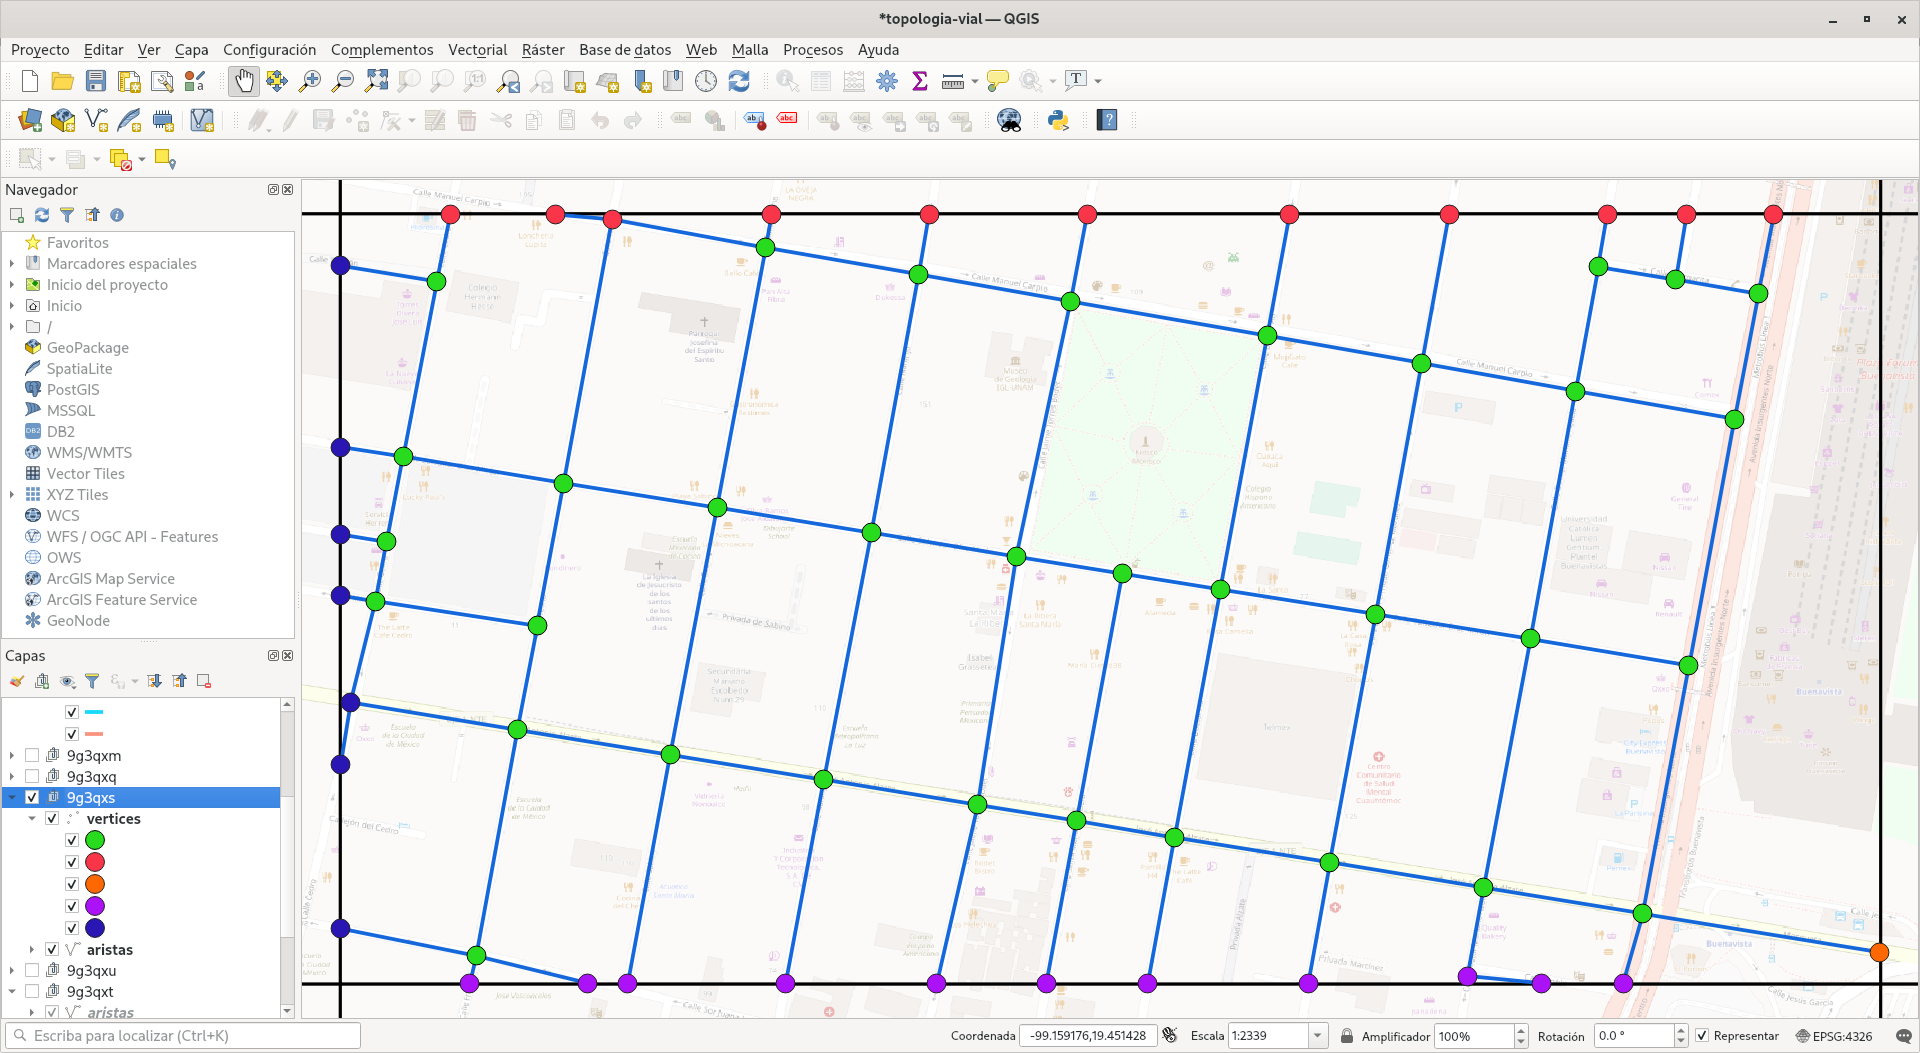
\includegraphics[width=1\textwidth]{qgis_grafo_vial}
\decoRule
\caption[Grafo vial en QGIS]{Grafo vial en QGIS.}
\label{fig:qgis_grafo_vial}
\end{figure}

Después, se creó el script
\href{https://gitlab.com/Comecacahuates/simulacion-protocolo-erutamiento/-/blob/main/scripts/shp2xml.py}{shp2xml.py}
para convertir cada par de archivos Shapefile en un archivo XML que contiene la
información de los vértices y las aristas de la red vial. Este script se
encuentra en el repositorio, y recibe como argumentos el directorio donde están
los archivos Shapefile, y el directorio donde se guardan los archivos XML, como
se muestra a continuación:

\begin{lstlisting}[language=bash]
$ scripts/shp2xml.py roadnetwork-database/shapefile \
    roadnetwork-database/xml
\end{lstlisting}

Los archivos XML se encuentran dentro del directorio
\code{roadnetwork-database/xml}, como se muestra a continuación:

\newpage

\dirtree{%
.1
\href{https://gitlab.com/Comecacahuates/simulacion-protocolo-erutamiento/-/tree/main/roadnetwork-database}{roadnetwork-database}.
  .2
  \href{https://gitlab.com/Comecacahuates/simulacion-protocolo-erutamiento/-/tree/main/roadnetwork-database/xml}{xml}.
    .3
    \href{https://gitlab.com/Comecacahuates/simulacion-protocolo-erutamiento/-/blob/main/roadnetwork-database/xml/9g3qxk.xml}{9g3qxk.xml}.
    .3
    \href{https://gitlab.com/Comecacahuates/simulacion-protocolo-erutamiento/-/blob/main/roadnetwork-database/xml/9g3qxm.xml}{9g3qxm.xml}.
    .3 
    \href{https://gitlab.com/Comecacahuates/simulacion-protocolo-erutamiento/-/blob/main/roadnetwork-database/xml/9g3qxq.xml}{9g3qxq.xml}.
    .3 \ldots.
}

El formato de los archivos XML de la base de datos es el siguiente:

\begin{lstlisting}[language=XML]
<?xml version="1.0" ?>
<roadnetwork>
  <vertices count="81">
    <vertex adjacency="3" id="0" lat="19.446251335" lon="-99.173579100"/>
    <vertex adjacency="2" id="1" lat="19.445807039" lon="-99.172773654"/>
    <vertex adjacency="-1" id="2" lat="19.446136882" lon="-99.172725752"/>
    ...
  </vertices>
  <edges count="105">
    <edge vertex-a="79" vertex-b="80"/>
    <edge vertex-a="80" vertex-b="78"/>
    <edge vertex-a="78" vertex-b="57"/>
    ...
  </edges>
</roadnetwork>
\end{lstlisting}

\section{Simulaciones de SUMO}
%-----------------------------------
%   SIMULACIÓNES DE SUMO
%-----------------------------------
\label{sec:simulaciones_sumo}

Para hacer una simulación del movimiento de los vehículos, primero se necesita
definir una red vial de SUMO por la que los vehículos puedan circular. Para
esto, primero se utilizó JOSM para descargar desde OpenStreetMap un archivo OSM
que contiene el mapa de la región de interés. Para descargar un mapa, se debe
que indicar la región delimitadora. En la figura
\ref{fig:josm_descargar_region}, se muestra cómo descargar la región Geohash
9g3qxs, cuyos límites en latitud son 19.4458007812 y 19.4512939453, y
en longitud son -99.1625976562 y -99.1516113281.

\begin{figure}[th!]
\centering
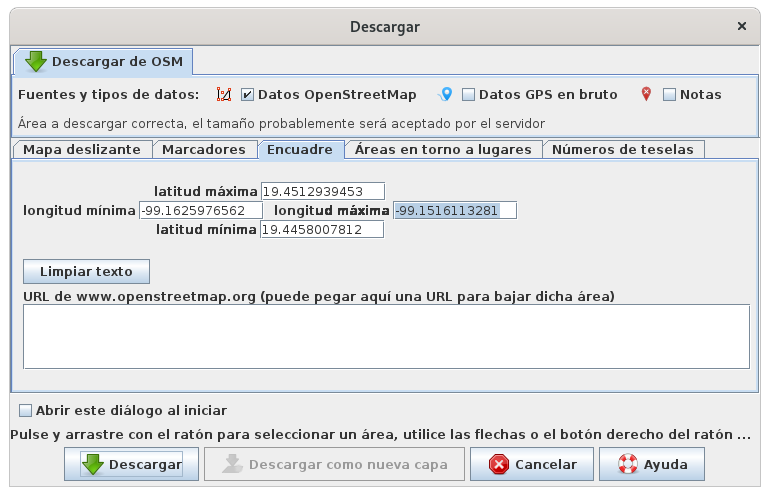
\includegraphics[width=1\textwidth]{josm_descargar_region}
\decoRule
\caption[Descargar mapa de la región Geohash 9g3qxs en JOSM]{Descargar mapa de
la región Geohash 9g3qxs en JOSM.}
\label{fig:josm_descargar_region}
\end{figure}

El mapa descargado incluye elementos fuera de la región de interés, como se
muestra en la figura \ref{fig:josm_mapa_descargado}. Es por esto que, se
utilizan las herramientas de JOSM para eliminar los elementos que son
innecesarios y recortar los segmentos de las vialidades que se encuentran fuera
de la región, así como corregir la cantidad de carriles de las calles. La
figura \ref{fig:josm_mapa_acondicionado} muestra el mapa después de realizar
este procedimiento, que se guarda con el nombre \code{9g3qxs.osm}.

\begin{figure}[th!]
\centering
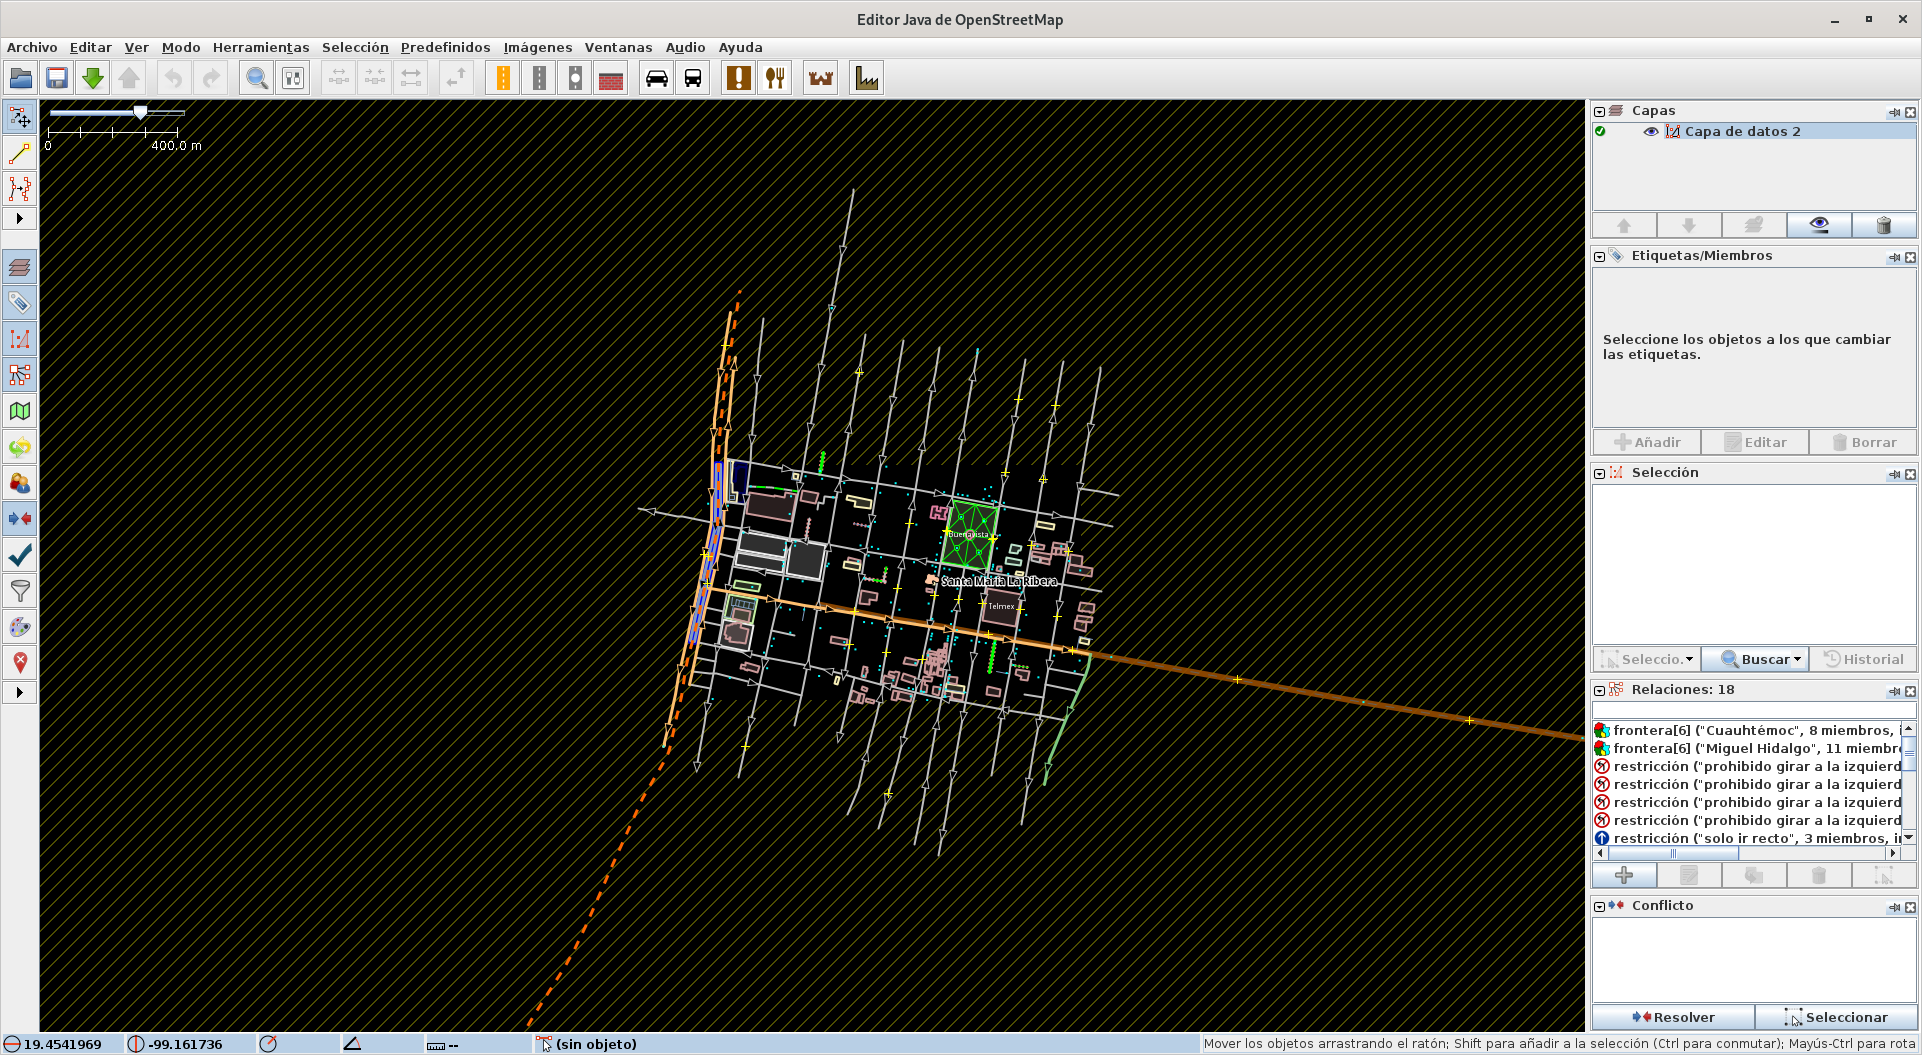
\includegraphics[width=1\textwidth]{josm_mapa_descargado} 
\decoRule
\caption[Mapa de la región Geohash 9g3qxs descargado con JOSM]{Mapa de la
región Geohash 9g3qxs descargado con JOSM.}
\label{fig:josm_mapa_descargado}
\end{figure}

\begin{figure}[th!]
\centering
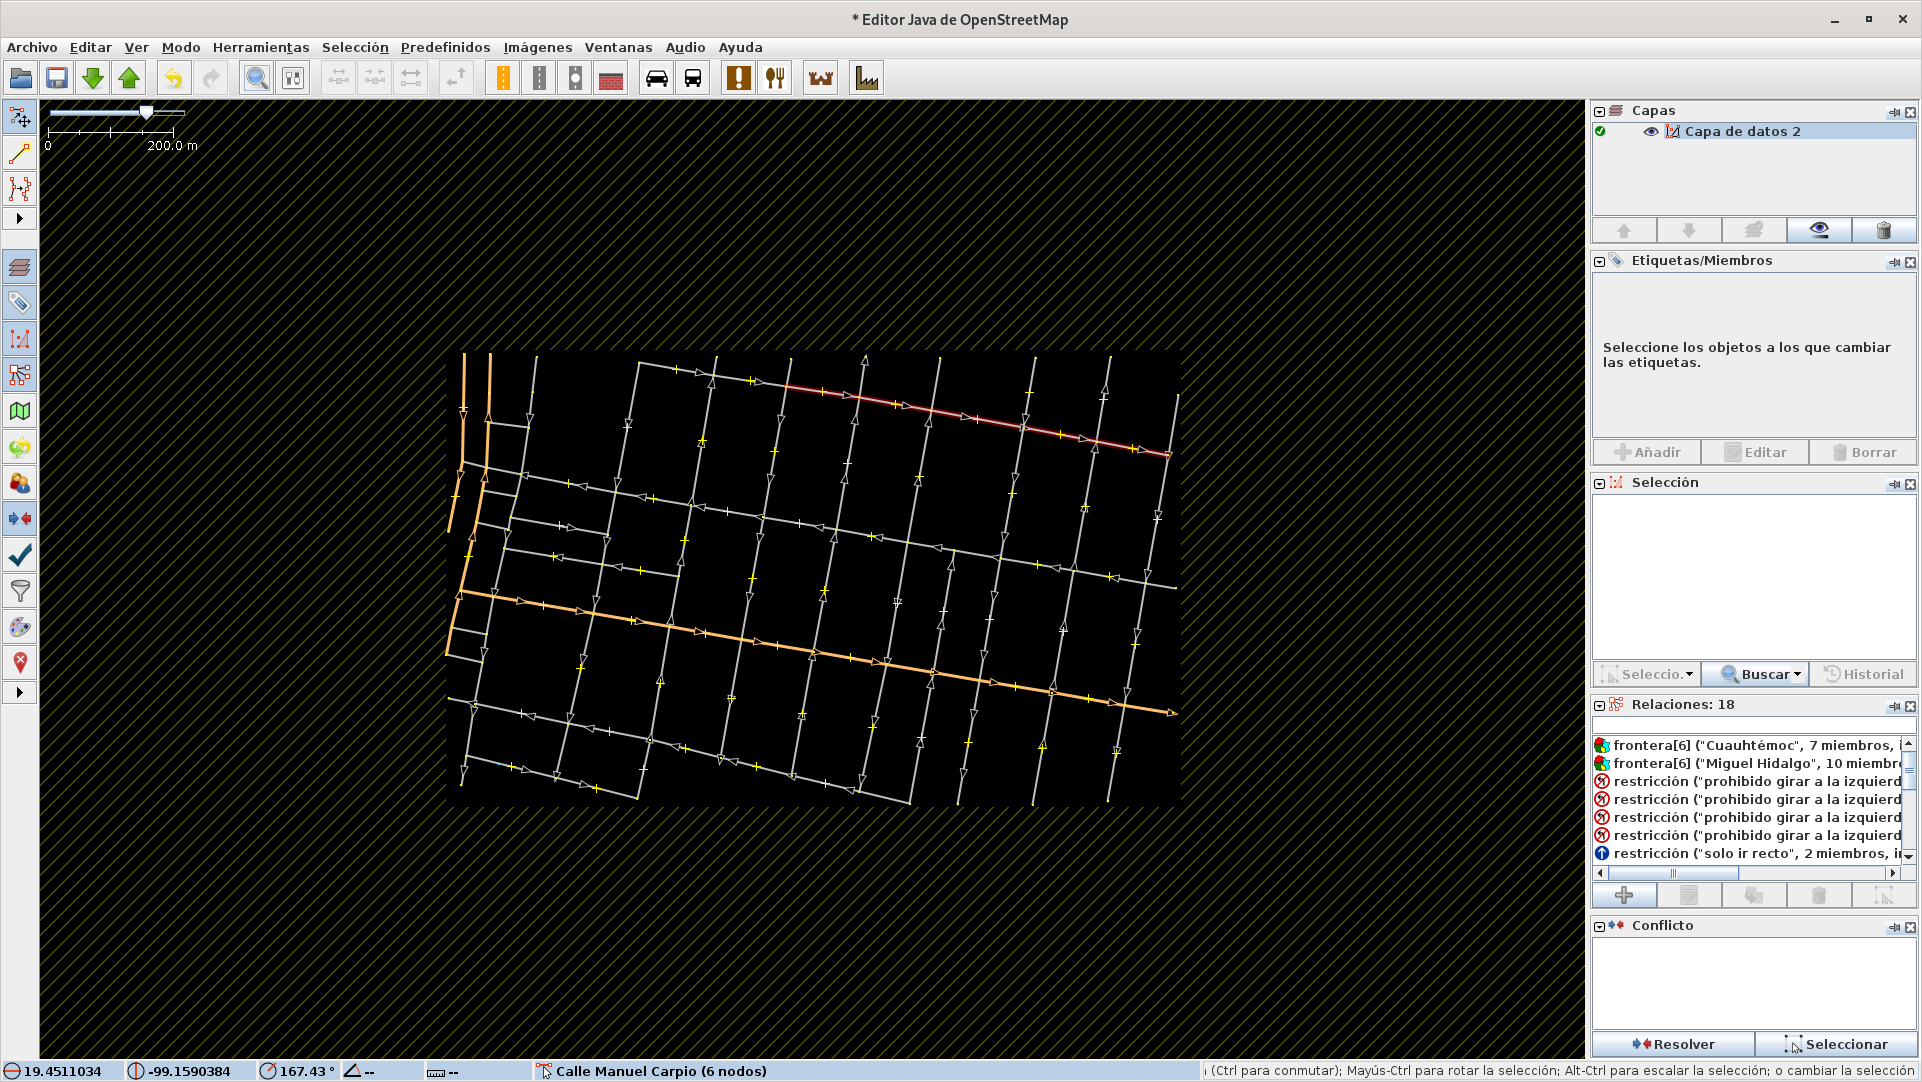
\includegraphics[width=1\textwidth]{josm_mapa_acondicionado}
\decoRule
\caption[Mapa de la región Geohash 9g3qxs acondicionado para la
simulación]{Mapa de la región Geohash 9g3qxs acondicionado para la simulación.}
\label{fig:josm_mapa_acondicionado}
\end{figure}

SUMO define su propio formato para representar las redes viales con archivos
XML (no confundir con los archivos XML de la base de datos de redes viales), y
cuenta con una herramienta llamada \code{netconvert}, cuyo objetivo es convertir
redes viales de diferentes formatos a redes viales de SUMO. Para obtener la red
de SUMO \code{9g3qxs.net.xml} a partir del mapa \code{9g3qxs.osm}, se ejecuta el
siguiente comando:

\begin{lstlisting}[language=bash]
$ netconvert --osm-files 9g3qxs.osm -o 9g3qxs.net.xml
\end{lstlisting}

Una vez que se cuenta con la red vial de SUMO, se necesita el modelo del tráfico
vehicular. SUMO proporciona diferentes herramientas y métodos para generar
estos modelos, y se pueden consultar en \cite{SUMOTrafico}. Teniendo el modelo
del tráfico en el archivo \code{9g3qxs.rou.xml}, se escribe el archivo de
configuración \code{9g3qxs.sumocfg.xml}, en el que se indica el archivo de la
red vial, el archivo del modelo del tráfico, los tiempos de inicio y final, y
demás parámetros de la simulación, como se muestra a continuación:

\begin{lstlisting}[language=XML]
<?xml version="1.0" ?>
<configuration>
    <input>
        <net-file value="9g3qxs.net.xml"/>
        <route-files value="9g3qxs.rou.xml"/>
    </input>
    <time>
        <begin value="0"/>
        <end value="60"/>
        <step-length value="0.1"/>
    </time>
</configuration>
\end{lstlisting}

Con el siguiente comando se ejecuta la simulación en modo gráfico:

\begin{lstlisting}[language=bash]
$ sumo-gui -c 9g3qxs.sumocfg
\end{lstlisting}

Al ejecutar la simulación, se muestra la red vial y una animación del
movimiento de los vehículos en el tiempo en una ventana como la que se muestra
en la figura \ref{fig:sumo_simulacion}. Este procedimiento se repite para
realizar todas las imulaciones necesarias, y estas se puede utilizar dentro de
la simulación de OMNeT++ mediante el uso de Veins.

\begin{figure}[th!]
\centering
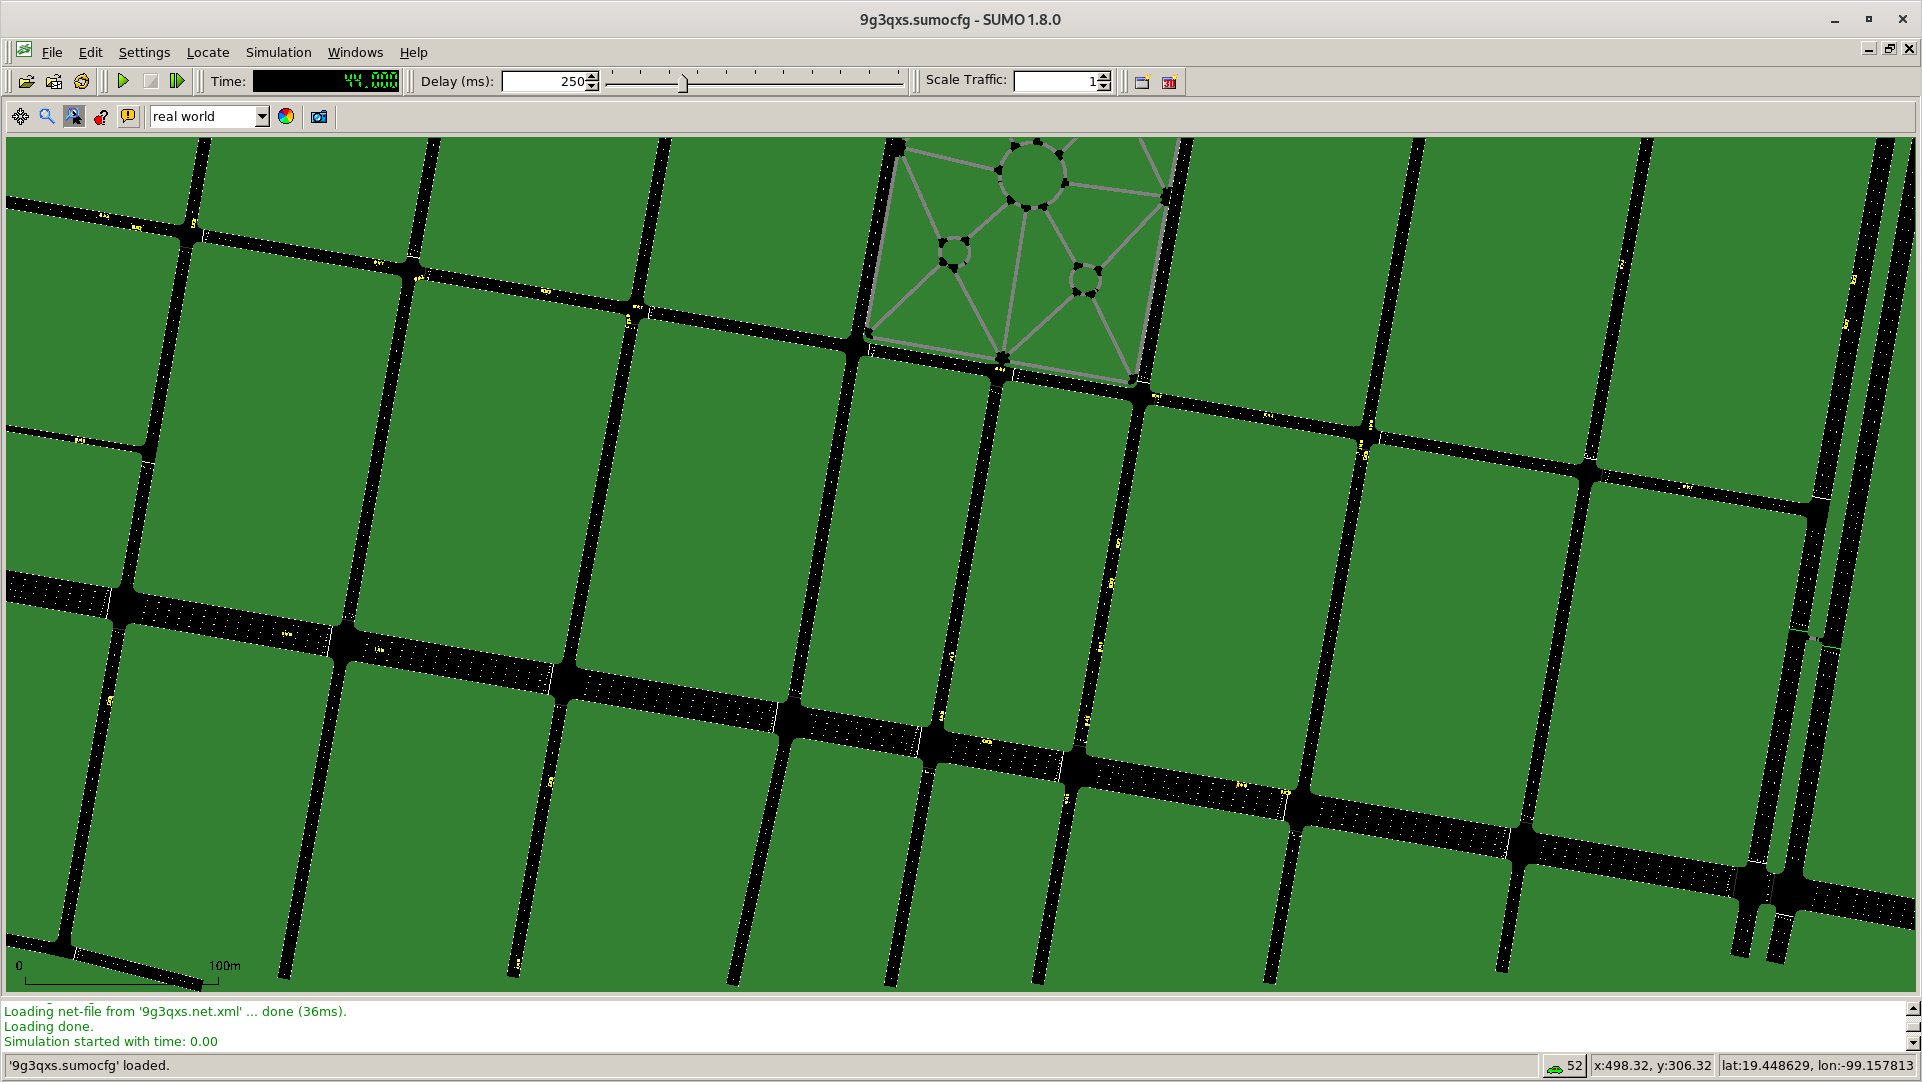
\includegraphics[width=1\textwidth]{sumo_simulacion}
\decoRule
\caption[Simulación de SUMO]{Simulación de SUMO.}
\label{fig:sumo_simulacion}
\end{figure}

\section{Proyecto de OMNeT++}
%-----------------------------------
%   PROYECTO DE OMNET++
%-----------------------------------
\label{sec:proyecto_omnet}

Para crear el proyecto de OMNeT++, primero se descarga
\href{https://inet.omnetpp.org/Download.html}{INET 4.3.1} y
\href{https://veins.car2x.org/download/}{Veins 5.1}, y se importan en OMNeT++.
Después, se crea el proyecto de OMNeT++ y se seleccionan los proyectos de INET y
Veins como dependencias.

Los proyectos en OMNeT++ se componen de módulos simples y compuestos, y estos
interactúan entre sí a lo largo del tiempo de simulación. Los módulos se definen
en un lenguaje llamado NED, que permite especificar sus parámetros para
modificar su comportamiento, además de compuertas mediante las cuales cada
módulo se comunica con otros. Los \keyword{módulos simples} se definen con un
archivo NED, y una clase de C++, donde se describe su comportamiento. Los
\keyword{módulos compuestos} se definen únicamente por un archivo NED, donde se
indica los módulos que lo componen y cómo se conectan entre ellos para
comunicarse.

A continuación, se explica la estructura del proyecto y cuáles son módulos más
importantes que lo componen. Las rutas de los directorios y archivos son
relativas a la raíz del repositorio. Por conveniencia, se utilizó una
nomenclatura similar a la que se utiliza en INET y Veins para los nombres de
los archivos y el código fuente.

\subsection{Base de datos de redes viales}
%-----------------------------------
%   BASE DE DATOS DE REDES VIALES
%-----------------------------------
\label{subsec:base_de_datos_de_redes_viales}

Como se mencionó en el capítulo \ref{ch:protocolo_de_enrutamiento_propuesto},
cada vehículo debe contar con una base de datos de redes viales. Sin embargo,
para optimizar los recursos de cómputo durante la simulación, únicamente hay un
módulo de base de datos de redes viales al que todos los vehículos tienen
acceso. Este módulo se define en los siguientes archivos:

\dirtree{%
.1
\href{https://gitlab.com/Comecacahuates/simulacion-protocolo-erutamiento/-/tree/main/src}{src}.
  .2
  \href{https://gitlab.com/Comecacahuates/simulacion-protocolo-erutamiento/-/tree/main/src/veins_proj}{veins\_proj}.
    .3
    \href{https://gitlab.com/Comecacahuates/simulacion-protocolo-erutamiento/-/tree/main/src/veins_proj/roadnetwork}{roadnetwork}.
      .4
      \href{https://gitlab.com/Comecacahuates/simulacion-protocolo-erutamiento/-/blob/main/src/veins_proj/roadnetwork/RoadNetworkGraph.h}{RoadNetworkGraph.h}.
      .4
      \href{https://gitlab.com/Comecacahuates/simulacion-protocolo-erutamiento/-/blob/main/src/veins_proj/roadnetwork/RoadNetworkGraph.cc}{RoadNetworkGraph.cc}.
      .4
      \href{https://gitlab.com/Comecacahuates/simulacion-protocolo-erutamiento/-/blob/main/src/veins_proj/roadnetwork/RoadNetwork.h}{RoadNetwork.h}.
      .4
      \href{https://gitlab.com/Comecacahuates/simulacion-protocolo-erutamiento/-/blob/main/src/veins_proj/roadnetwork/RoadNetwork.cc}{RoadNetwork.cc}.
      .4
      \href{https://gitlab.com/Comecacahuates/simulacion-protocolo-erutamiento/-/blob/main/src/veins_proj/roadnetwork/RoadNetworkDatabase.ned}{RoadNetworkDatabase.ned}.
      .4
      \href{https://gitlab.com/Comecacahuates/simulacion-protocolo-erutamiento/-/blob/main/src/veins_proj/roadnetwork/RoadNetworkDatabase.h}{RoadNetworkDatabase.h}.
      .4
      \href{https://gitlab.com/Comecacahuates/simulacion-protocolo-erutamiento/-/blob/main/src/veins_proj/roadnetwork/RoadNetworkDatabase.cc}{RoadNetworkDatabase.cc}.
}

En \code{RoadNetworkGraph.h}, se declaran los tipos de datos para la creación de
los grafos, además de algunas funciones útiles relacionadas con estos. Para la
implementación de los grafos, se utilizó la biblioteca Boost \cite{Boost}.

En \code{RoadNetwork.h} y \code{RoadNetwork.cc}, se define la clase
\code{RoadNetwork}, que se encarga de crear un grafo a partir de un archivo XML
de la base de datos de grafos viales. Además incluye métodos para calcular la
ubicación vial de los vehículos, calcular el peso de una arista y calcular la
ruta más corta.

\begin{sloppypar}
El módulo \code{RoadNetworkDatabase} es global, y lee los archivos XML de la
base de datos de redes viales, y crea un objeto de la clase \code{RoadNetwork} a
partir de cada archivo. Su comportamiento se describe en
\code{RoadNetworkDatabase.h} y \code{RoadNetworkDatabase.cc}.
\end{sloppypar}

\subsection{Movilidad de los nodos}
%-----------------------------------
%   MOVILIDAD DE LOS NODOS
%-----------------------------------
\label{subsec:movilidad_de_los_nodos}

Cada nodo de la red necesita tener un módulo de movilidad, que permita, entre
otras cosas, conocer su ubicación. Es por esto, que se creó un módulo de
movilidad para los vehículos y uno para los \textit{hosts}. Estos se definen en
los siguiente archivos:

\dirtree{%
.1
\href{https://gitlab.com/Comecacahuates/simulacion-protocolo-erutamiento/-/tree/main/src}{src}.
  .2
  \href{https://gitlab.com/Comecacahuates/simulacion-protocolo-erutamiento/-/tree/main/src/veins_proj}{veins\_proj}.
    .3
    \href{https://gitlab.com/Comecacahuates/simulacion-protocolo-erutamiento/-/tree/main/src/veins_proj/mobility}{mobility}.
      .4
      \href{https://gitlab.com/Comecacahuates/simulacion-protocolo-erutamiento/-/blob/main/src/veins_proj/mobility/StaticHostMobility.ned}{StaticHostMobility.ned}.
      .4
      \href{https://gitlab.com/Comecacahuates/simulacion-protocolo-erutamiento/-/blob/main/src/veins_proj/mobility/StaticHostMobility.h}{StaticHostMobility.h}.
      .4
      \href{https://gitlab.com/Comecacahuates/simulacion-protocolo-erutamiento/-/blob/main/src/veins_proj/mobility/StaticHostMobility.cc}{StaticHostMobility.cc}.
      .4
      \href{https://gitlab.com/Comecacahuates/simulacion-protocolo-erutamiento/-/blob/main/src/veins_proj/mobility/CarMobility.ned}{CarMobility.ned}.
      .4
      \href{https://gitlab.com/Comecacahuates/simulacion-protocolo-erutamiento/-/blob/main/src/veins_proj/mobility/CarMobility.h}{CarMobility.h}.
      .4
      \href{https://gitlab.com/Comecacahuates/simulacion-protocolo-erutamiento/-/blob/main/src/veins_proj/mobility/CarMobility.cc}{CarMobility.cc}.
}

\begin{sloppypar}
Debido a que los \textit{hosts} son estáticos, su módulo de movilidad
\code{StaticHostMobility} hereda del módulo
\href{https://doc.omnetpp.org/inet/api-current/neddoc/inet.mobility.static.StationaryMobility.html}{\code{StationaryMobility}}
de INET. Este módulo establece la ubicación geográfica inicial del
\textit{host}, y permite acceder a esta.
\end{sloppypar}

\begin{sloppypar}
Por otro lado, la ubicación de los vehículos cambia de acuerdo a la simulación
de SUMO. Es por esto que se creó el módulo \code{CarMobility}, que hereda del
módulo
\href{https://veins.car2x.org/documentation/modules/#veins_inet}{\code{VeinsInetMobility}},
proporcionado por Veins, para obtener información del estatus del vehículo. El
módulo \code{CarMobility} permite acceder a la ubicación geográfica, velocidad y
dirección de movimiento de un vehículo, así como la red vial en la que se
encuentra y su ubicación vial dentro de esta.
\end{sloppypar}

\subsection{Servicio de localización}
%-----------------------------------
%   SERVICIO DE LOCALIZACIÓN
%-----------------------------------
\label{subsec:servicio_de_localizacion_sim}

Desarrollar un servicio de localización está fuera del alcance de este trabajo.
Sin embargo, cada \textit{host} necesita conocer la ubicación de todos los demás
para poder comunicarse con ellos. Por este motivo, se implementó un servicio de
localización muy simple con el único propósito de cubrir esta necesidad en la
simulación. Este se define en los siguientes archivos:

\dirtree{%
.1
\href{https://gitlab.com/Comecacahuates/simulacion-protocolo-erutamiento/-/tree/main/src}{src}.
  .2
  \href{https://gitlab.com/Comecacahuates/simulacion-protocolo-erutamiento/-/tree/main/src/veins_proj}{veins\_proj}.
    .3
  \href{https://gitlab.com/Comecacahuates/simulacion-protocolo-erutamiento/-/tree/main/src/veins_proj/locationservice}{locationservice}.
      .4
      \href{https://gitlab.com/Comecacahuates/simulacion-protocolo-erutamiento/-/blob/main/src/veins_proj/locationservice/HostsLocationTable.ned}{HostsLocationTable.ned}.
      .4
      \href{https://gitlab.com/Comecacahuates/simulacion-protocolo-erutamiento/-/blob/main/src/veins_proj/locationservice/HostsLocationTable.h}{HostsLocationTable.h}.
      .4
      \href{https://gitlab.com/Comecacahuates/simulacion-protocolo-erutamiento/-/blob/main/src/veins_proj/locationservice/HostsLocationTable.cc}{HostsLocationTable.cc}.
}

\begin{sloppypar}
El módulo \code{HostsLocationTable} es un módulo global que contiene la
dirección IP \textit{unicast} de cada \textit{host} y su ubicación. Cuando el
módulo \code{StaticHostConfigurator} de un \textit{host} realiza la
configuración de la interfaz, también registra su dirección \textit{unicast} y
su ubicación en el módulo \code{HostsLocationTable}. Cuando un \textit{host}
necesita conocer la ubicación de otro para enviarle un paquete, la obtiene del
módulo \code{HostsLocationTable}.
\end{sloppypar}

\subsection{Autoconfiguración de direcciones}
%-----------------------------------
%   AUTOCONFIGURACIÓN DE DIRECCIONES
%-----------------------------------
\label{subsec:autoconfiguracion_de_direcciones_sim}

Para implementar el protocolo de autoconfiguración de direcciones, se crearos
dos módulos, uno para los vehículos y uno para los \textit{hosts}. Estos se
definen en los siguientes archivos:

\dirtree{%
.1
\href{https://gitlab.com/Comecacahuates/simulacion-protocolo-erutamiento/-/tree/main/src}{src}.
  .2
  \href{https://gitlab.com/Comecacahuates/simulacion-protocolo-erutamiento/-/tree/main/src/veins_proj}{veins\_proj}.
    .3
    \href{https://gitlab.com/Comecacahuates/simulacion-protocolo-erutamiento/-/tree/main/src/veins_proj/networklayer}{networklayer}.
      .4
    \href{https://gitlab.com/Comecacahuates/simulacion-protocolo-erutamiento/-/tree/main/src/veins_proj/networklayer/ipv6}{ipv6}.
        .5
      \href{https://gitlab.com/Comecacahuates/simulacion-protocolo-erutamiento/-/blob/main/src/veins_proj/networklayer/ipv6/Ipv6GeohashAddress.h}{Ipv6GeohashAddress.h}.
        .5
      \href{https://gitlab.com/Comecacahuates/simulacion-protocolo-erutamiento/-/blob/main/src/veins_proj/networklayer/ipv6/Ipv6GeohashAddress.cc}{Ipv6GeohashAddress.cc}.
      .4
    \href{https://gitlab.com/Comecacahuates/simulacion-protocolo-erutamiento/-/tree/main/src/veins_proj/networklayer/configurator}{configurator}.
        .5
      \href{https://gitlab.com/Comecacahuates/simulacion-protocolo-erutamiento/-/blob/main/src/veins_proj/networklayer/configurator/StaticHostConfigurator.ned}{StaticHostConfigurator.ned}.
        .5
      \href{https://gitlab.com/Comecacahuates/simulacion-protocolo-erutamiento/-/blob/main/src/veins_proj/networklayer/configurator/StaticHostConfigurator.h}{StaticHostConfigurator.h}.
        .5
      \href{https://gitlab.com/Comecacahuates/simulacion-protocolo-erutamiento/-/blob/main/src/veins_proj/networklayer/configurator/StaticHostConfigurator.cc}{StaticHostConfigurator.cc}.
        .5
      \href{https://gitlab.com/Comecacahuates/simulacion-protocolo-erutamiento/-/blob/main/src/veins_proj/networklayer/configurator/CarConfigurator.ned}{CarConfigurator.ned}.
        .5
      \href{https://gitlab.com/Comecacahuates/simulacion-protocolo-erutamiento/-/blob/main/src/veins_proj/networklayer/configurator/CarConfigurator.h}{CarConfigurator.h}.
        .5
      \href{https://gitlab.com/Comecacahuates/simulacion-protocolo-erutamiento/-/blob/main/src/veins_proj/networklayer/configurator/CarConfigurator.cc}{CarConfigurator.cc}.
}

En \code{Ipv6GeohashAddress.h} e \code{Ipv6GeohashAddress.cc} se incluyen
funciones que generan direcciones IPv6 \textit{unicast} y \textit{multicast}
a partir de códigos Geohash (sección \ref{sec:formato_direcciones_ipv6}).

Para la autoconfiguración de \textit{hosts}, se creó el módulo
\code{StaticHostConfigurator}, que obtiene la ubicación del \textit{host}
mediante el módulo \code{StaticHostMobility}, y crea las direcciones
\textit{unicast} y \textit{multicast} y las asigna a la interfaz. Debido a que
los \textit{hosts} no se mueven, este procedimiento se realiza sólo una vez para
cada uno.

Para el caso de los vehículos, se creó el módulo \code{CarConfigurator}. Este
solicita periódicamente la ubicación del vehículo al módulo \code{CarMobility},
y, si es necesario, crea las direcciones \textit{unicast} y \textit{multicast} y
asignarlas a la interfaz. Además, este módulo se encarga de realizar el
procedimiento de cambio de subred (sección \ref{sec:cambio_subred}).

\subsection{Protocolo de enrutamiento}
%-----------------------------------
%   PROTOCOLO DE ENRUTAMIENTO
%-----------------------------------
\label{subsec:protocolo_de_enrutamiento_sim}

Los vehículos y \textit{hosts} tienen un módulo que se encarga de realizar el
proceso de enrutamiento del protocolo propuesto (capítulo
\ref{ch:protocolo_de_enrutamiento_propuesto}). Estos se definen en los
siguientes archivos:

\dirtree{%
.1
\href{https://gitlab.com/Comecacahuates/simulacion-protocolo-erutamiento/-/tree/main/src}{src}.
  .2
  \href{https://gitlab.com/Comecacahuates/simulacion-protocolo-erutamiento/-/tree/main/src/veins_proj}{veins\_proj}.
    .3
    \href{https://gitlab.com/Comecacahuates/simulacion-protocolo-erutamiento/-/tree/main/src/veins_proj/routing}{routing}.
      .4
      \href{https://gitlab.com/Comecacahuates/simulacion-protocolo-erutamiento/-/blob/main/src/veins_proj/routing/Routing.msg}{Routing.msg}.
      .4
      \href{https://gitlab.com/Comecacahuates/simulacion-protocolo-erutamiento/-/blob/main/src/veins_proj/routing/RoutingProtocolBase.ned}{RoutingProtocolBase.ned}.
      .4
      \href{https://gitlab.com/Comecacahuates/simulacion-protocolo-erutamiento/-/blob/main/src/veins_proj/routing/RoutingProtocolBase.h}{RoutingProtocolBase.h}.
      .4
      \href{https://gitlab.com/Comecacahuates/simulacion-protocolo-erutamiento/-/blob/main/src/veins_proj/routing/RoutingProtocolBase.cc}{RoutingProtocolBase.cc}.
      .4
      \href{https://gitlab.com/Comecacahuates/simulacion-protocolo-erutamiento/-/blob/main/src/veins_proj/routing/StaticHostRoutingProtocol.ned}{StaticHostRoutingProtocol.ned}.
      .4
      \href{https://gitlab.com/Comecacahuates/simulacion-protocolo-erutamiento/-/blob/main/src/veins_proj/routing/StaticHostRoutingProtocol.h}{StaticHostRoutingProtocol.h}.
      .4
      \href{https://gitlab.com/Comecacahuates/simulacion-protocolo-erutamiento/-/blob/main/src/veins_proj/routing/StaticHostRoutingProtocol.cc}{StaticHostRoutingProtocol.cc}.
      .4
      \href{https://gitlab.com/Comecacahuates/simulacion-protocolo-erutamiento/-/blob/main/src/veins_proj/routing/CarRoutingProtocol.ned}{CarRoutingProtocol.ned}.
      .4
      \href{https://gitlab.com/Comecacahuates/simulacion-protocolo-erutamiento/-/blob/main/src/veins_proj/routing/CarRoutingProtocol.h}{CarRoutingProtocol.h}.
      .4
      \href{https://gitlab.com/Comecacahuates/simulacion-protocolo-erutamiento/-/blob/main/src/veins_proj/routing/CarRoutingProtocol.cc}{CarRoutingProtocol.cc}.
}

Los mensajes de enrutamiento (sección \ref{sec:mensajes_de_enrutamiento})
y las opciones de la cabecera de opciones de salto (sección
\ref{sec:cabecera_opciones}) se definen en \code{Routing.msg}.

Los \textit{hosts} y los vehículos no realizan exactamente las mismas
operaciones durante el enrutamiento. Es por esto que se definió el módulo
\code{RoutingProtocolBase}, que implementa las operaciones de enrutamiento
comunes para los dos tipos de nodos, como el directorio de vehículos vecinos
(sección \ref{sec:directiorio_vehiculos_vecinos}) y la depuración de las rutas
expiradas. Este módulo también define los parámetros de configuración del
protocolo (sección \ref{sec:lista_de_parametros_de_configuracion}).

\begin{sloppypar}
El módulo \code{StaticHostRoutingProtocol} hereda del módulo
\code{RoutingProtocolBase}, e implementa la transmisión de mensajes
\mbox{HOLA\_HOST} (sección \ref{subsec:mensaje_hola_host}), así como seleccionar
el vehículo más cercano como siguiente salto para cada paquete.
\end{sloppypar}

\begin{sloppypar}
El módulo \code{CarRoutingProtocol} hereda del módulo
\code{RoutingProtocolBase}, e implementa la transmisión de mensajes
\mbox{HOLA\_VEHIC} (sección \ref{subsec:mensaje_hola_vehic}) y el directorio de \textit{hosts}
vecinos (sección \ref{sec:directorio_hosts_vecinos}).
Además, este módulo se encarga del cálculo de rutas viales, determinar el vértice de destino
local y seleccionar el siguiente salto para cada paquete (secciones
\ref{sec:enrutamiento_vial}, \ref{sec:computo_rutas_viales} y
\ref{sec:seleccion_siguiente_salto}).
\end{sloppypar}

\subsection{Nodos de la red}
%-----------------------------------
%   NODOS DE LA RED
%-----------------------------------
\label{subsec:nodos_de_la_red_sim}

INET proporciona modelos base para nodos de una red, como el módulo
\href{https://doc.omnetpp.org/inet/api-current/neddoc/inet.node.inet.AdhocHost.html}{\code{AdhocHost}},
que incluyen módulos como protocolos de comunicación, tablas de enrutamiento,
tablas de interfaces, movilidad, etc. Para representar los vehiculos y
\textit{hosts} de la VANET, se crearon dos módulos a partir de este, que se
definen en los siguientes archivos:

\dirtree{%
.1
\href{https://gitlab.com/Comecacahuates/simulacion-protocolo-erutamiento/-/tree/main/src}{src}.
  .2
  \href{https://gitlab.com/Comecacahuates/simulacion-protocolo-erutamiento/-/tree/main/src/veins_proj}{veins\_proj}.
    .3
    \href{https://gitlab.com/Comecacahuates/simulacion-protocolo-erutamiento/-/tree/main/src/veins_proj/node}{node}.
      .4
      \href{https://gitlab.com/Comecacahuates/simulacion-protocolo-erutamiento/-/blob/main/src/veins_proj/node/StaticHost.ned}{StaticHost.ned}.
      .4
      \href{https://gitlab.com/Comecacahuates/simulacion-protocolo-erutamiento/-/blob/main/src/veins_proj/node/Car.ned}{Car.ned}.
}

\begin{sloppypar}
El módulo \code{StaticHost} incluye los módulos \code{StaticHostMobility},
\code{StaticHostConfigurator} y \code{RoutingProtocolStaticHost}, y su
estructura se muestra en la figura \ref{fig:static_host}. De manera similar, el
módulo \code{Car} incluye los módulos \code{CarMobility}, \code{CarConfigurator}
y \code{RoutingProtocolCar}, y su estructura se muestra en la figura
\ref{fig:car}.
\end{sloppypar}

\begin{figure}[th!]
\centering
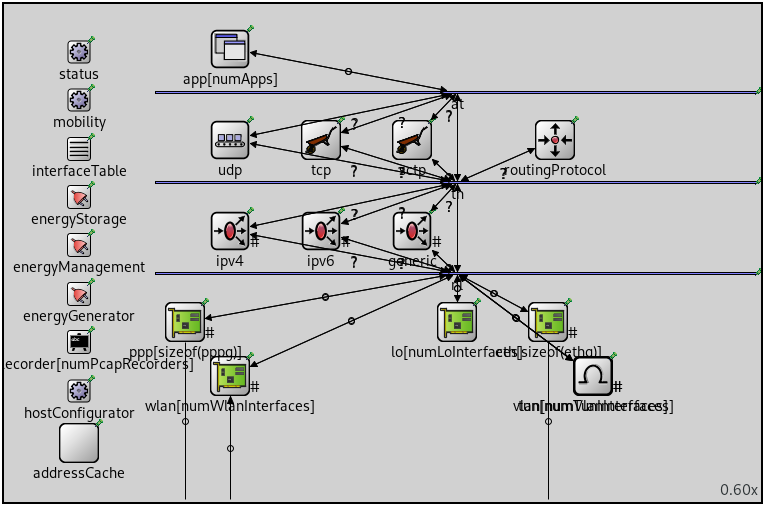
\includegraphics[width=1\textwidth]{static_host}
\decoRule
\caption[Estructura del módulo \code{StaticHost}]{Estructura del módulo
\code{StaticHost}.}
\label{fig:static_host}
\end{figure}

\begin{figure}[th!]
\centering
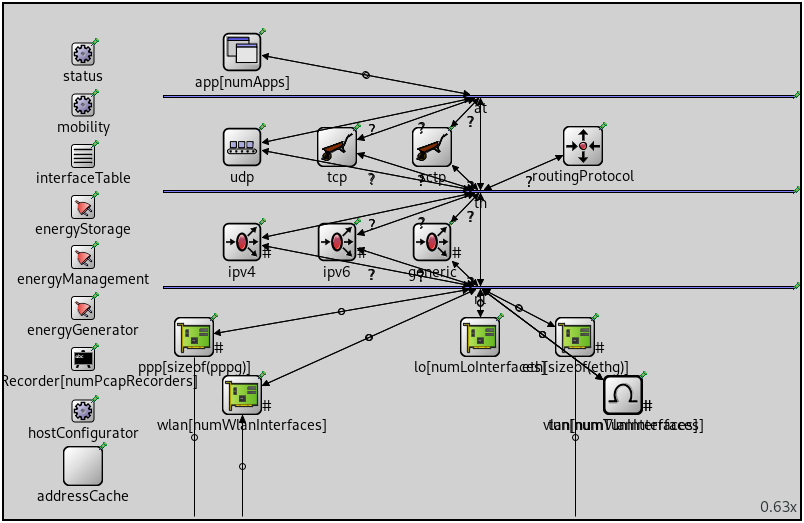
\includegraphics[width=1\textwidth]{car}
\decoRule
\caption[Estructura del módulo \code{Car}]{Estructura del módulo \code{Car}.}
\label{fig:car}
\end{figure}
